
% crash2.tex: created 2019-10-21 from minimal.tex for a 2 hour minicourse.

\documentclass[12pt, a4paper]{article}

\raggedbottom

\RequirePackage[l2tabu, orthodox]{nag}

\usepackage[top=20mm,bottom=20mm,left=25mm,right=25mm]{geometry}

\usepackage{showkeys}

\usepackage{amsmath,amssymb,amsfonts}

\usepackage{centernot}

\usepackage{underbracket}

\usepackage[nottoc]{tocbibind}

\usepackage{pgf}
\usepackage{tikz}

\usepackage{multirow}

\usepackage{pgf}
\usepackage{tikz}

\usepackage{xcolor}

% Syntax: \colorboxed[<color model>]{<color specification>}{<math formula>}
\newcommand*{\colorboxed}{}
\def\colorboxed#1#{%
  \colorboxedAux{#1}%
}
\newcommand*{\colorboxedAux}[3]{%
  % #1: optional argument for color model
  % #2: color specification
  % #3: formula
  \begingroup
    \colorlet{cb@saved}{.}%
    \color#1{#2}%
    \boxed{%
      \color{cb@saved}%
      #3%
    }%
  \endgroup
}

\usepackage[most]{tcolorbox}

\tcbset{
    frame code={}
    center title,
    left=0pt,
    right=0pt,
    top=0pt,
    bottom=0pt,
    colback=green!15,
    colframe=white,
    % width=\dimexpr\textwidth\relax,
    enlarge left by=0mm,
    % boxsep=5pt,
    arc=0pt,outer arc=0pt,
    breakable,
    }

\usepackage{amsthm}

\usepackage{thmtools}
%\usepackage{thm-restate}   This package does not interact very smoothly with \theoremstyle and \listoftheorems

\makeatletter
% \def\@endtheorem{\endtrivlist\@endpefalse }% OLD
\def\@endtheorem{\endtrivlist}% NEW
\makeatother

\newtheoremstyle{break}{9pt}{9pt}{\itshape}{}{\bfseries}{}{\newline}{}
\theoremstyle{break}    

\newtheorem{exo}{Exercise}[section]
\newtheorem{hyp}[exo]{Axiom}
\newtheorem{res}[exo]{Result}
\newtheorem{defn}[exo]{Definition}

\usepackage[colorlinks=true,linktoc=all,linkcolor=black,citecolor=red,urlcolor=blue]{hyperref}

\title{\bfseries Introduction to two-dimensional \\ conformal field theory}

\author{Sylvain Ribault \vspace{2mm}
\\
{\normalsize CEA Saclay, Institut de Physique Th\'eorique}
 \\
 {\footnotesize \ttfamily sylvain.ribault@ipht.fr }
}

\begin{document}

\maketitle

\begin{abstract}
I will review the basic principles of two-dimensional conformal field theory, and some important results. First I will explain the origin and consequences of the existence of a Virasoro symmetry algebra. Then I will sketch the conformal boostrap approach to conformal field theory. Finally I will introduce minimal models and Liouville theory, and sketch how their spectrums and correlation functions can be computed exactly. (This is an abridged version of my minimal lectures \href{https://arxiv.org/abs/1609.09523}{\texttt arXiv:1609.09523}, written for a mini-course that should last about two hours.)
\end{abstract}

%\clearpage

\tableofcontents

\hypersetup{linkcolor=blue}

\numberwithin{equation}{section}
\setcounter{section}{-1}

\section{Introduction}

Two-dimensional CFTs belong to the rare cases of quantum field theories that can be exactly solved, thanks to their infinite-dimensional symmetry algebras. They are interesting for their applications to statistical physics, they are the technical basis of string theory in the worldsheet approach, and they can guide the exploration of higher-dimensional CFTs. 

We will introduce the main ideas of two-dimensional CFT in the conformal bootstrap approach, and focus on the simplest nontrivial models that have been solved: minimal models and Liouville theory. 
The conformal bootstrap is an axiomatic approach, where the main objects are correlation functions. 
Fields are just notations for writing axioms on correlation functions, and only make sense in the context of correlation functions.

\section{The Virasoro algebra and its representations}

\subsection{Algebra}

By definition, conformal transformations are transformations that preserve angles. 
In two dimensions with a complex coordinate $z$, any holomorphic transformation preserves angles.
Infinitesimal conformal transformations are holomorphic functions close to the identity function, 
\begin{align}
 z \mapsto z + \epsilon z^{n+1}\qquad (n\in\mathbb{Z}\ , \ \epsilon\ll 1) \ .
\end{align}
These transformations act on functions of $z$ via the differential operators 
\begin{align}
 \ell_n = -z^{n+1}\frac{\partial}{\partial z}\ ,
\end{align}
and these operators generate the Witt algebra, with commutation relations
\begin{align}
 [\ell_n,\ell_m ] = (n-m)\ell_{m+n}\ .
\end{align}

%\begin{tcolorbox}
The generators $(\ell_{-1},\ell_0,\ell_1)$ generate a subalgebra called the algebra of infinitesimal global conformal transformations and isomorphic to $s\ell_2$.  The corresponding Lie group is the group of global conformal transformations of 
the Riemann sphere $\mathbb{C}\cup \{\infty\}$,
\begin{align}
 z \mapsto \frac{az+b}{cz+d}\quad , \quad (a,b,c,d\in \mathbb{C},\ ad-bc\neq 0)\ .
\end{align}

In a quantum theory, symmetry transformations act projectively on states. 
Projective representations of an algebra are equivalent to representations of a centrally extended algebra. 
This is why we always look for central extensions of symmetry algebras.

\begin{defn}[Virasoro algebra]
 ~\label{def:vir}
 The central extension of the Witt algebra is called the Virasoro algebra. It has the generators $(L_n)_{n\in\mathbb{Z}}$ and $\mathbf 1$, and the commutation relations
 \begin{align}
  [\mathbf 1, L_n] = 0 \quad , \quad [L_n,L_m] = (n-m)L_{n+m} +\frac{c}{12}(n-1)n(n+1)\delta_{n+m,0}\mathbf 1 \ ,
  \label{eq:vir}
 \end{align}
 where the number $c$ is called the central charge. (The notation $c\mathbf 1$ stands for a central generator that always has the same eigenvalue $c$ within a given conformal field theory.)
\end{defn}

\subsection{Representations}

The spectrum, i.e. the space of states, must be a representation of the Virasoro algebra. Let us now make assumptions on what type of representation it can be.

\begin{hyp}[Representations that can appear in the spectrum]
 ~\label{hyp:rep}
 The spectrum is a direct sum of irreducible representations. In the spectrum, $L_0$ is diagonalizable, and the real part of its eigenvalues is bounded from below.
\end{hyp}
Why this special role for $L_0$? Because we want to interpret it as the energy operator. 
The $L_0$ eigenvalue of an $L_0$ eigenvector is called its conformal dimension. The action of $L_n$ shifts conformal dimensions by $-n$:
\begin{align}
 L_0|v\rangle = \Delta|v\rangle \quad \Rightarrow\quad  
 L_0 L_n|v\rangle 
 = (\Delta-n)L_n|v\rangle \ .
\end{align}
From our axiom, we deduce that any irreducible representation is generated by its state with the lowest conformal dimension, which is a primary state.

\begin{defn}[Primary and descendant states, level, Verma module]
 ~\label{def:prim}
 A primary state with conformal dimension $\Delta$ is a state $|v\rangle\neq 0$ such that 
 \begin{align}
  L_0 |v\rangle = \Delta |v\rangle \quad , \quad L_{n>0} |v\rangle = 0\ .
 \end{align}
The Verma module $\mathcal V_\Delta$ is the representation whose basis is 
 $
 \left\{ \prod_{i=1}^k L_{-n_i} |v\rangle\right\}_{ 0<n_1\leq \dots \leq n_k}
 $.
The state $\prod_{i=1}^k L_{-n_i} |v\rangle $ has the conformal dimension $\Delta+N$, where $N=\sum_{i=1}^k n_i\geq 0$ is called the level. A state of level $N\geq 1$ is called a descendant state.
\end{defn}
Let us plot a basis of primary and descendant states up to the level $3$:
\begin{align}
 \begin{tikzpicture}[scale = .25, baseline=(current  bounding  box.center)]
  \draw[-latex, very thick] (20, 0) -- (20, -21) node [right] {$N$};
  \foreach \x in {0, ..., 3}
  {
  \draw [dotted] (-20, {-6*\x}) -- (20, {-6*\x}) node [right] {${\x}$};
  }
  \node[fill = white] at (0, 0) (0) {$|v\rangle$};
  \node[fill = white] at (-4,-6) (1) {$L_{-1}|v\rangle$};
  \node[fill = white] at (-8, -12) (11) {$L_{-1}^2|v\rangle$};
  \node[fill = white] at (-12, -18) (111) {$L_{-1}^3|v\rangle$};
  \node[fill = white] at (0,-12) (2) {$L_{-2}|v\rangle$};
  \node[fill = white] at (0,-18) (12) {$L_{-1}L_{-2}|v\rangle$};
  \node[fill = white] at (8,-18) (3) {$L_{-3}|v\rangle$};
  \draw[-latex] (0) -- (1);
  \draw[-latex] (1) -- (11);
  \draw[-latex] (11) -- (111);
  \draw[-latex] (0) -- (2);
  \draw[-latex] (0) -- (3);
  \draw[-latex] (2) -- (12);
 \end{tikzpicture}
\end{align}
We need not include the state $L_{-2}L_{-1}|v\rangle$, due to $L_{-2}L_{-1} = L_{-1}L_{-2} - L_{-3}$.

\subsection{Null vectors and degenerate representations}\label{sec:nv}

A Verma module is irreducible if and only if it has no null vector.

\begin{defn}[Null vectors]
 ~\label{def:nv}
 A descendant state that is also primary is called a null vector or singular vector.
\end{defn}
In the Verma module $\mathcal V_\Delta$, let us look for null vectors at the level $N=1$. For $n\geq 1$ we have 
\begin{align}
L_n L_{-1}|v\rangle = [L_n, L_{-1}] |v\rangle = (n+1) L_{n-1}|v\rangle = 
\left\{\begin{array}{ll} 0 &  \quad \text{if } n\geq 2\ , \\ 2\Delta |v\rangle & \quad \text{if } n = 1\ . \end{array}\right. 
\end{align}
So $L_{-1}|v\rangle$ is a null vector if and only if $\Delta=0$, and the Verma module $\mathcal V_0$ is reducible.
At level $N=2$, there exists a null vector of the form $|\chi\rangle = (L_{-1}^2 + a L_{-2})|v\rangle$ if and only if 
 \begin{align}
 \Delta = \frac{1}{16}\left( 5-c\pm\sqrt{(c-1)(c-25)} \right) \ .
 \label{eq:dpm}
\end{align}
In order to simplify this formula, let us introduce other notations for $c$ and $\Delta$. We define
\begin{align}
 \text{the background charge } Q \ , & \quad c = 1+6Q^2\ , \quad \text{up to } Q \mapsto -Q\ ,
 \label{eq:cqb}
 \\
 \text{the coupling constant } b \ , & \quad Q = b+\frac{1}{b} \ , \quad \text{up to } b\mapsto \pm b^{\pm 1}\ ,
 \\
 \text{the momentum } P\  , &\quad \Delta = \frac{Q^2}{4}-P^2\ , \quad \text{up to reflections } P \mapsto -P\ .
\label{eq:refm}
 \end{align}
The condition \eqref{eq:dpm} for the existence of a level two null vector becomes 
\begin{align}
 P = \frac12\left( b+ b^{-1} + b^{\pm 1}\right)\ .
\end{align}
Let us summarize the momentums of the Verma modules that have null vectors at levels $N=1,2$, and the null vectors themselves:
\begin{align}
\renewcommand{\arraystretch}{1.3}
\begin{array}{|c|c|c|c|}
\hline 
N & \langle r,s\rangle & P_{\langle r,s\rangle} &  L_{\langle r,s\rangle} 
\\
\hline\hline
1 & \langle 1,1\rangle & \frac12\left(b+b^{-1}\right) &  L_{-1}
\\
\hline
\multirow{2}{*}{2} & 
\langle 2,1\rangle & \frac12\left( 2b+ b^{-1}\right)  & L_{-1}^2 + b^2 L_{-2}
\\
\cline{2-4}
& \langle 1,2\rangle & \frac12\left( b+ 2b^{-1} \right) & L_{-1}^2 + b^{-2} L_{-2} 
\\
\hline
rs & \langle r,s\rangle &  \frac12\left(rb+sb^{-1}\right) & L_{-1}^{rs} + \cdots 
\\
\hline
\end{array}
\label{eq:ars}
\end{align}
The generalization to higher levels $N\geq 3$ is that the dimensions of Verma modules with null vectors are labelled by positive integers $r,s$ such that $N=rs$. We write these dimensions $\Delta_{\langle r,s\rangle}$, and the corresponding momentums $P_{\langle r,s\rangle}$. 

If $\Delta\notin\{\Delta_{\langle r,s\rangle}\}_{r,s\in\mathbb{N}^*}$, then $\mathcal V_\Delta$ is irreducible. If $\Delta = \Delta_{\langle r,s\rangle}$, then $\mathcal V_\Delta$ contains a nontrivial submodule, generated by the null vector and its descendant states. For generic values of the central charge $c$, this submodule is the Verma module $\mathcal V_{\Delta_{\langle r,s\rangle}+rs}$.

\begin{defn}[Degenerate representation]
 ~\label{def:deg}
The coset of the reducible Verma module $\mathcal V_{\Delta_{\langle r,s\rangle}}$ by its Verma submodule $\mathcal V_{\Delta_{\langle r,s\rangle}+rs}$ is an irreducible module $\mathcal{R}_{\langle r,s\rangle}$, which is called a degenerate representation:
\begin{align}
 \mathcal{R}_{\langle r,s\rangle} = \frac{\mathcal V_{\Delta_{\langle r,s\rangle}}}{\mathcal V_{\Delta_{\langle r,s\rangle}+rs}}\ .
\end{align}
In this representation, the null vector vanishes,
\begin{align}
 L_{\langle r,s\rangle}|v\rangle = 0\ .
\end{align}
\end{defn}


\section{Correlation functions and fields}\label{sec:cft}

\subsection{Definition}

In the conformal bootstrap approach, the basic objects are correlation functions. An $N$-point correlation function is a function of $N$ positions $z_1,\cdots,z_N$, written as 
\begin{align}
  \Big< V_1(z_1) \cdots V_N(z_N) \Big>\ .
 \end{align}
It also depends on the central charge $c$, and on the nature of the fields $V_1,\cdots V_N$. Fields and correlation functions are defined by a number of axioms. To begin with, correlation functions depend linearly on fields, and in particular $\frac{\partial}{\partial z_1} \left< V_1(z_1) \cdots V_N(z_N) \right> = \left< \frac{\partial}{\partial z_1}V_1(z_1) \cdots V_N(z_N) \right>$. 

\begin{hyp}[Commutativity of fields]
 ~\label{hyp:ass}
 Correlation functions do not depend on the order of the fields,
 \begin{align}
  V_1(z_1) V_2(z_2) = V_2(z_2)V_1(z_1)\ .
 \end{align}
\end{hyp}

\begin{hyp}[Action of the Virasoro algebra]
~\label{hyp:vaf}
 The Virasoro algebra acts on fields: $V(z) \mapsto L_n^{(z)}V(z)=L_n V(z)$. This action is such that for any field,
 \begin{align}
  \frac{\partial}{\partial z} V(z) = L_{-1}^{(z)} V(z)  \ .
  \label{pvlv}
 \end{align}
It follows that the following expression is $z$-independent,
 \begin{align}
  T(y) = \sum_{n\in\mathbb{Z}} \frac{L_n^{(z)}}{(y-z)^{n+2}} \ .
 \end{align}
 This is called the energy-momentum tensor, and is itself considered as a field.
\end{hyp}

\begin{defn}[Primary field, descendant field, degenerate field]
~\label{def:pfdf}
A primary field $V_\Delta(z)$ of conformal dimension $\Delta$ is a field such that 
\begin{align}
 L_0 V_\Delta(z) = \Delta V_\Delta(z) \quad , \quad  L_{n> 0} V_\Delta(z) = 0 \ .
\end{align}
A degenerate field $V_{\langle r,s\rangle}(z)$ corresponds to the primary state of the degenerate representation $\mathcal{R}_{\langle r,s\rangle}$, and therefore obeys 
\begin{align}
L_0 V_{\langle r,s\rangle}(z) = \Delta_{\langle r,s\rangle} V_{\langle r,s\rangle}(z) \quad , \quad  L_{n> 0} V_{\langle r,s\rangle}(z) = 0 \quad , \quad L_{\langle r, s\rangle} V_{\langle r,s\rangle}(z) = 0\ .
\end{align}
\end{defn}
It follows that 
\begin{align}
 T(y)V_\Delta(z)= \sum_{n\in\mathbb{Z}} \frac{L_n V_\Delta(z)}{(y-z)^{n+2}} \underset{y\to z}{=} \frac{\Delta}{(y-z)^2} V_\Delta(z) + \frac{1}{y-z} \frac{\partial}{\partial z} V_\Delta(z) + O(1)\ . 
 \label{eq:tvd}
\end{align}
This is a particular case of an operator product expansion.


\subsection{Dependence on positions}

From our axioms, we can deduce that correlation functions of primary fields have a simple behaviour under global conformal transformations,
\begin{align}
 \left< \prod_{i=1}^N  V_{\Delta_i}\left(\frac{az_i+b}{cz_i+d}\right) \right>
 = \prod_{i=1}^N (cz_i +d)^{2\Delta_i} \left< \prod_{i=1}^N V_{\Delta_i}(z_i) \right>\ .
 \label{eq:zgc}
\end{align}
In the case of two-point functions, this implies
\begin{align}
 \Big< V_{\Delta_1}(z_1)V_{\Delta_2}(z_2) \Big> \propto \delta_{\Delta_1,\Delta_2} (z_1-z_2)^{-2\Delta_1} \ .
 \label{eq:2pt}
\end{align}
So a two-point function can be non-vanishing only if the two fields have the same dimension.
For three-point functions, this implies
\begin{align}
 \left< \prod_{i=1}^3 V_{\Delta_i}(z_i) \right> \propto (z_1-z_2)^{\Delta_3-\Delta_1-\Delta_2} (z_1-z_3)^{\Delta_2-\Delta_1-\Delta_3} (z_2-z_3)^{\Delta_1-\Delta_2-\Delta_3}\ ,
 \label{eq:3pt}
\end{align}
with an unknown proportionality coefficient that does not depend on $z_i$.
For four-point functions, the general solution can be written as 
\begin{align}
 \left< \prod_{i=1}^4 V_{\Delta_i}(z_i) \right> 
 = z_{13}^{-2\Delta_1} z_{23}^{\Delta_1-\Delta_2-\Delta_3+\Delta_4} z_{24}^{-\Delta_1-\Delta_2+\Delta_3-\Delta_4} z_{34}^{\Delta_1+\Delta_2-\Delta_3-\Delta_4} G\left(\frac{z_{12}z_{34}}{z_{13}z_{24}}\right)\ ,
 \label{eq:4pt}
\end{align}
where $z_{ij} = z_i - z_j$ and $G(z)$ is an arbitrary function of the cross-ratio $z$. 
So conformal symmetry reduces the four-point function to a function of one variable $G$ -- equivalently, we can set $z_2,z_3,z_4$ to fixed values, and recover the four-point function from its dependence on $z_1$ alone. In particular,
 \begin{align}
  G(z) = \Big< V_{\Delta_1}(z) V_{\Delta_2}(0)V_{\Delta_3}(\infty)V_{\Delta_4}(1) \Big>\ .
 \end{align}

We have been studying global conformal invariance of correlation functions of primary fields, rather than more general fields. This was not only for making things simpler, but also because correlation functions of descendants can be deduced from correlation functions of primaries. For example,
\begin{align}
 \Big< L_{-2}V_{\Delta_1}(z_1) \cdots V_{\Delta_N}(z_N) \Big>
  =\sum_{i=2}^N\left(\frac{1}{z_1-z_i}\frac{\partial}{\partial z_i} +\frac{\Delta_i}{(z_i-z_1)^2}\right)  \Big< V_{\Delta_1}(z_1) \cdots V_{\Delta_N}(z_N)\Big>\ .
  \label{eq:ltv}
\end{align}


\subsection{Belavin--Polyakov--Zamolodchikov equations}

Consider an $N$-point function of primary field, where one field is moreover degenerate, say $V_{\langle 2, 1 \rangle}(z_1)$. By definition,
\begin{align}
\left(L_{-1}^2 + b^2 L_{-2}\right) V_{\langle 2, 1 \rangle}(z_1)  = 0\qquad \text{so that} \qquad L_{-2}V_{\langle 2, 1 \rangle}(z_1) = -\frac{1}{b^2}\frac{\partial^2}{\partial z_1^2} V_{\langle 2, 1 \rangle}(z_1)\ .
\end{align}
Using the identity \eqref{eq:ltv},
this leads to the second-order Belavin--Polyakov--Zamolodchikov partial differential equation
\begin{align}
 \left( \frac{1}{b^2}\frac{\partial^2}{\partial z_1^2} + \sum_{i=2}^N\left(\frac{1}{z_1-z_i}\frac{\partial}{\partial z_i} +\frac{\Delta_i}{(z_1-z_i)^2}\right) \right)\left< V_{\langle 2, 1 \rangle}(z_1) \prod_{i=2}^N V_{\Delta_i}(z_i) \right>  = 0\ .
 \label{eq:bpz}
\end{align}
More generally, a correlation function with the degenerate field $V_{\langle r,s\rangle}$ obeys a partial differential equation of order $rs$. 

In the case of a three-point function, the dependence on $z_i$ is already completely determined by conformal symmetry, and the BPZ equation leads to constraints on the conformal dimensions:
\begin{align}
 \left< V_{\langle 2, 1 \rangle} V_{\Delta_2} V_{\Delta_3} \right> \neq 0 \quad \implies \quad 
 P_2 = P_3 \pm \frac{b}{2}\ .
 \label{eq:alpm}
\end{align}
In the case of a four-point function, the BPZ equation amounts to a hypergeometric differential equation for the function of one variable $G(z)$.


\section{Conformal bootstrap}

We have seen how conformal symmetry leads to linear equations for correlation functions.
In order to fully determine correlation functions, we need additional, nonlinear equations, and therefore additional axioms: single-valuedness of correlation functions, and existence of operator product expansions.  

\subsection{Single-valuedness}\label{sec:sv}

\begin{hyp}[Single-valuedness]
 ~\label{hyp:sv}
 Correlation functions are single-valued functions of the positions, i.e. they have trivial monodromies.
\end{hyp}
Our two-point function \eqref{eq:2pt} however has nontrivial monodromy unless $\Delta_1\in \frac12\mathbb{Z}$, as a  result of solving holomorphic Ward identities. 
We would rather have a single-valued function of the type $|z_1-z_2|^{-4\Delta_1} = (z_1-z_2)^{-2\Delta_1} (\bar z_1-\bar z_2)^{-2\Delta_1}$.
This suggests that we need antiholomorphic Ward identities as well, and therefore a second copy of the Virasoro algebra.

\begin{hyp}[Left and right Virasoro algebras]
 ~\label{hyp:lr}
 We have two mutually commuting Virasoro symmetry algebras with the same central charge, called left-moving or holomorphic, and right-moving or antiholomorphic. Their generators are written $L_n,\bar L_n$, with in particular
 \begin{align}
  \frac{\partial}{\partial z} V(z) = L_{-1}V(z)   \quad , \quad \frac{\partial}{\partial \bar z} V(z)= \bar L_{-1} V(z)   \ .
 \end{align}
 The generators of conformal transformations are the diagonal combinations $L_n+\bar L_n$.
\end{hyp}
Let us consider left- and right-primary fields $V_{\Delta_i,\bar\Delta_i}(z_i)$, with the 
two-point functions
\begin{align}
 \left<\prod_{i=1}^2 V_{\Delta_i,\bar\Delta_i}(z_i) \right> \propto \delta_{\Delta_1,\Delta_2}\delta_{\bar\Delta_1,\bar\Delta_2} (z_1-z_2)^{-2\Delta_1} (\bar z_1-\bar z_2)^{-2\bar\Delta_1}\ .
\end{align}
This is single-valued if and only if our two fields have half-integer spins,
\begin{align}
 \Delta -\bar \Delta \in \frac12\mathbb{Z}\ .
\end{align} 
The simplest case is $\Delta=\bar\Delta$, which leads to the definition

\begin{defn}[Diagonal states, diagonal fields and diagonal spectrums]
 ~\label{def:diag}
 A primary state or field is called diagonal if it has the same left and right conformal dimensions. A spectrum is called diagonal if all primary states are diagonal.
\end{defn}
For diagonal primary fields, we will now write  $V_\Delta(z) = V_{\Delta,\Delta}(z)$.


\subsection{Operator product expansion and crossing symmetry}

\begin{hyp}[Operator product expansion]
 ~\label{hyp:ope}
 For any two fields $V_1,V_2$, there exist coefficients $C^i_{12}(z_1,z_2)$ such that we have the operator product expansion (OPE) 
 \begin{align}
  V_{1}(z_1)V_{2}(z_2) \underset{z_1\to z_2}{=} \sum_i C^i_{12}(z_1,z_2) V_{i}(z_2)\ ,
 \end{align}
 where the sum is over all fields in the theory.
 In a correlation function,
 this sum converges for $z_1$ sufficiently close to $z_2$.
\end{hyp}

If the spectrum is made of diagonal primary states and their descendant states, the OPE of two primary fields is
\begin{align}
 V_{\Delta_1}(z_1) V_{\Delta_2}(z_2) 
\underset{z_1\to z_2}{=} \sum_{\Delta\in S} C_{\Delta_1,\Delta_2,\Delta} |z_1-z_2|^{2(\Delta-\Delta_1-\Delta_2)}
 \Big(V_{\Delta}(z_2) + O(z_1-z_2) \Big)\ ,
 \label{eq:ope}
\end{align}
where $S$ is a set of conformal dimensions called the spectrum,
and the subleading terms are contributions of descendant fields. 
In particular, the $z_1,z_2$-dependence of the coefficients is dictated by the behaviour
of correlation functions under translations $z_i\to z_i+c$ and dilations $z_i\to\lambda z_i$, leaving a $z_i$-independent unknown coefficient $C_{\Delta_1,\Delta_2,\Delta}$.
Assuming the two-point function is normalized as $\left< V_{\Delta}(z_1)V_{\Delta}(z_2) \right> = |z_1-z_2|^{-4\Delta}$, this factor is the three-point structure constant such that 
\begin{align}
 \left<\prod_{i=1}^3 V_{\Delta_i}(z_i) \right> = C_{\Delta_1,\Delta_2,\Delta_3} |z_1-z_2|^{2(\Delta_3-\Delta_1-\Delta_2)} |z_1-z_3|^{2(\Delta_2-\Delta_1-\Delta_3)} |z_2-z_3|^{2(\Delta_1-\Delta_2-\Delta_3)}\ ,
\end{align}

Using the OPE, we can decompose a four-point function of primary fields into structure constants and conformal blocks,
\begin{align}
\Big<V_{\Delta_1}(z)V_{\Delta_2}(0)V_{\Delta_3}(\infty)V_{\Delta_4}(1)\Big>
 =\sum_{\Delta\in S} C_{\Delta_1,\Delta_2,\Delta} C_{\Delta,\Delta_3,\Delta_4}  \mathcal{F}^{(s)}_\Delta(z) \mathcal{F}^{(s)}_\Delta(\bar z)\ .
 \label{sdec}
\end{align}

\begin{defn}[Conformal block]
 ~\label{def:block}
 The four-point conformal block on the sphere,
 \begin{align}
  \mathcal{F}^{(s)}_\Delta(z) \underset{z\to 0}{=} z^{\Delta-\Delta_1-\Delta_2}\left( 1 + \frac{(\Delta+\Delta_1-\Delta_2)(\Delta+\Delta_4-\Delta_3)}{2\Delta}z + O(z^2) \right)\ ,
  \label{eq:gsd}
 \end{align}
is the normalized contribution of the Verma module $\mathcal V_\Delta$ to a four-point function, obtained by summing over left-moving descendants. It is a locally holomorphic function of $z$. Its dependence on $c,\Delta_1,\Delta_2,\Delta_3,\Delta_4$ are kept implicit. The label $(s)$ stands for $s$-channel.
\end{defn}
Conformal blocks are in principle known, as they are universal functions, entirely determined by conformal symmetry. 
This is analogous to characters of representations, also known as zero-point conformal blocks on the torus.

Our axiom \ref{hyp:ass} on the commutativity of fields implies that the OPE is associative, and that we can use the OPE of any two fields in a four-point function. In particular, using the OPE of the first and fourth fields, we obtain 
\begin{align}
 \Big<V_{\Delta_1}(z)V_{\Delta_2}(0)V_{\Delta_3}(\infty)V_{\Delta_4}(1)\Big>
 =\sum_{\Delta\in S} C_{\Delta,\Delta_1,\Delta_4} C_{\Delta_2,\Delta_3,\Delta}   \mathcal{F}^{(t)}_\Delta(z) \mathcal{F}^{(t)}_\Delta(\bar z)\ ,
 \label{tdec}
\end{align}
where $\mathcal{F}^{(t)}_\Delta(z) \underset{z\to 1}{=} (z-1)^{\Delta-\Delta_1-\Delta_4}\Big(1+O(z-1)\Big)$ is a $t$-channel conformal block.
The equality of our two decompositions \eqref{sdec} and \eqref{tdec} of the four-point function is called crossing symmetry, schematically 
\begin{align}
 \sum_{\Delta_s\in S} C_{12s} C_{s34} 
 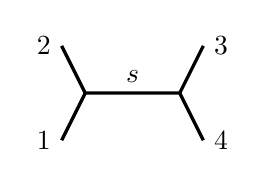
\begin{tikzpicture}[baseline=(current  bounding  box.center), very thick, scale = .3]
\draw (-1,2) node [left] {$2$} -- (0,0) -- node [above] {$s$} (4,0) -- (5,2) node [right] {$3$};
\draw (-1,-2) node [left] {$1$} -- (0,0);
\draw (4,0) -- (5,-2) node [right] {$4$};
\end{tikzpicture} 
= \sum_{\Delta_t\in S} C_{23t}C_{t41} 
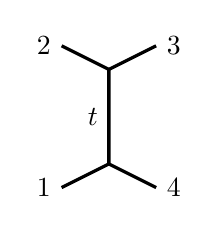
\begin{tikzpicture}[baseline=(current  bounding  box.center), very thick, scale = .3]
 \draw (-2,3) node [left] {$2$} -- (0,2) -- node [left] {$t$} (0,-2) -- (-2, -3) node [left] {$1$};
\draw (0,2) -- (2,3) node [right] {$3$};
\draw (0,-2) -- (2, -3) node [right] {$4$};
\end{tikzpicture}
\ .
\label{csd}
\end{align}
The unknowns in this equation are the spectrum $S$ and three-point structure constant $C$. 
Any solution such that $C$ is invariant under permutations allows us to consistently compute arbitrary correlation functions on the sphere, not just four-point functions.

\begin{defn}[Conformal field theory]
~\label{def:cft}
A (model of) conformal field theory on the Riemann sphere is a spectrum $S$ and a permutation-invariant three-point structure constant $C$ that obey crossing symmetry.
\end{defn}


\subsection{Degenerate fields and the fusion product}\label{sec:dffp}

Crossing symmetry equations are powerful, but typically involve infinite sums, which makes them difficult to solve.
However, if at least one field is degenerate, then the four-point function belongs to the finite-dimensional space of solutions of a BPZ equation, and is therefore a combination of finitely many conformal blocks. 
For example,
$G(z)=\Big< V_{\langle 2, 1 \rangle}(z) V_{\Delta_1}(0)V_{\Delta_2}(\infty)V_{\Delta_3}(1) \Big>$ is a combination of only two holomorphic $s$-channel conformal blocks.
These two blocks are characterized by their asymptotic behaviour near $z=0$ \eqref{eq:gsd}, where the BPZ equation allows only two values of $\Delta$, namely $\Delta\in\{\Delta(P_1-\frac{b}{2}),\Delta(P_1+\frac{b}{2})\}$.
Another basis of solutions of the same BPZ equation is given by two $t$-channel blocks, which are characterized by their power-like behaviour near $z=1$.
\begin{align}
 \mathcal{F}^{(s)}_\pm(z)  =  
 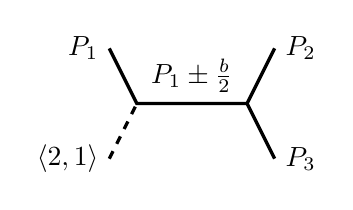
\begin{tikzpicture}[baseline=(current  bounding  box.center), very thick, scale = .35]
\draw (-1,2) node [left] {$P_1$} -- (0,0) -- node [above] {$P_1\pm \frac{b}{2}$} (4,0) -- (5,2) node [right] {$P_2$};
\draw[dashed] (-1,-2) node [left] {$\langle 2,1 \rangle$} -- (0,0);
\draw (4,0) -- (5,-2) node [right] {$P_3$};
\end{tikzpicture}
\qquad , \qquad 
\mathcal{F}^{(t)}_\pm(z)  =  
 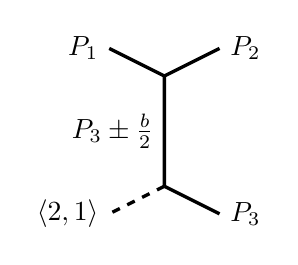
\begin{tikzpicture}[baseline=(current  bounding  box.center), very thick, scale = .35]
 \draw (-2,3) node [left] {$P_1$} -- (0,2) -- node [left] {$P_3\pm \frac{b}{2}$} (0,-2);
 \draw[dashed] (0, -2) -- (-2, -3) node [left] {$\langle 2,1 \rangle$};
\draw (0,2) -- (2,3) node [right] {$P_2$};
\draw (0,-2) -- (2, -3) node [right] {$P_3$};
\end{tikzpicture}
\label{gpic}
\end{align}
Let us build single-valued four-point functions as linear combinations of such blocks. Single-valuedness near $z=0$ forbids terms such as $\mathcal{F}^{(s)}_{-}(z) \mathcal{F}^{(s)}_{+}(\bar z)$, and we must have 
\begin{align}
 G(z) = \sum_{\epsilon=\pm} c^{(s)}_{\epsilon} \mathcal{F}^{(s)}_{\epsilon}(z) \mathcal{F}^{(s)}_{\epsilon}(\bar z) = \sum_{\eta=\pm} c^{(t)}_{\eta} \mathcal{F}^{(t)}_{\eta}(z) \mathcal{F}^{(t)}_{\eta}(\bar z)\ .
 \label{gz}
\end{align}
The $s$- and $t$-channel blocks are two bases of the same space of solutions of the BPZ equation, and they are linearly related,
\begin{align}
 \mathcal{F}^{(s)}_{\epsilon}(z) = \sum_{\eta=\pm} F_{\epsilon\eta} \mathcal{F}^{(t)}_{\eta}(z)\ .
\end{align}
In particular, this implies 
\begin{align}
 \frac{c_{+}^{(s)}}{c_{-}^{(s)}} = -\frac{F_{-+}F_{--}}{F_{++}F_{+-}} \ .
 \label{eq:coc}
\end{align}
We will later express $c_\pm^{(s)}$ in terms of three-point structure constants, and obtain equations for these structure constants.

The presence of only two $s$-channel fields with momentums $P_1\pm \frac{b}{2}$ means that the operator product expansion $V_{\langle 2, 1 \rangle}(z) V_{P_1}(0)$ involves only two primary fields $V_{P_1\pm \frac{b}{2}}(0)$. 

\begin{defn}[Fusion product]
 ~\label{def:fus}
 The fusion product is a bilinear product of representations of the Virasoro algebra, that encodes the constraints on OPEs from Virasoro symmetry and null vectors. In particular,
 \begin{align}
  \mathcal{R}_{\langle 1,1\rangle}\times \mathcal V_P = \mathcal V_P \quad , \quad 
  \mathcal{R}_{\langle 2,1\rangle}\times \mathcal V_P = \sum_\pm \mathcal V_{P\pm \frac{b}{2}}\quad , \quad  
  \mathcal{R}_{\langle 1,2\rangle}\times \mathcal V_P = \sum_\pm \mathcal V_{P\pm \frac{1}{2b}}\ .
  \label{eq:rv}
 \end{align}
 From the commutativity of fields, it follows that the fusion product is commutative and associative.
\end{defn}
Using associativity, we can work out the fusion products (and even the existence) of higher degenerate representations, for example, 
\begin{align}
 \mathcal{R}_{\langle 2,1\rangle}\times \mathcal{R}_{\langle 2,1\rangle} = \mathcal{R}_{\langle 1,1\rangle} + \mathcal{R}_{\langle 3,1\rangle} \quad , \quad \mathcal{R}_{\langle 3,1\rangle} \times \mathcal V_P = \mathcal V_{P - b} + \mathcal V_P + \mathcal V_{P + b}\ .
\end{align}
More generally, the degenerate representations $\mathcal{R}_{\langle r,s \rangle}$ have the fusion products
 \begin{align}
 \mathcal{R}_{\langle r,s \rangle}\times \mathcal{V}_P &= \mathcal{R}_{\langle r,s \rangle}\times \mathcal{V}_P = \sum_{i=-\frac{r-1}{2}}^{\frac{r-1}{2}} \sum_{j=-\frac{s-1}{2}}^{\frac{s-1}{2}} \mathcal{V}_{P + ib+jb^{-1}}\ ,
\label{rtv}
 \\
 \mathcal{R}_{\langle r_1,s_1 \rangle} \times \mathcal{R}_{\langle r_2,s_2 \rangle} &= \sum_{r_3\overset{2}{=}|r_1-r_2|+1}^{r_1+r_2-1}\ \sum_{s_3\overset{2}{=}|s_1-s_2|+1}^{s_1+s_2-1} \mathcal{R}_{\langle r_3,s_3 \rangle}\ ,
\label{rrsr}
\end{align}
where the sums run by increments of $2$ if there is a superscript in $\overset{2}{=}$, and $1$ otherwise.

\section{Minimal models}

\begin{defn}[Minimal model]
 ~\label{def:mm}
 A minimal model is a conformal field theory whose spectrum is made of finitely many irreducible representations of the product of the left and the right Virasoro algebras.
\end{defn}

\subsection{Diagonal minimal models}\label{sec:amm}

We first focus on diagonal minimal models, whose spectrums are of the type
\begin{align}
 S = \bigoplus_\mathcal{R} \mathcal{R}\otimes  \mathcal{\bar R}\ ,
\end{align}
where $\mathcal{R}$ and $ \mathcal{\bar R}$ denote the same Virasoro representation, viewed as a representation of the left- or right-moving Virasoro algebra respectively.

\begin{hyp}[Degenerate spectrum]
 ~\label{hyp:deg}
 All representations that appear in the spectrum of a minimal model are degenerate.
\end{hyp}
It is natural to use degenerate representations, because in an OPE of degenerate fields, only finitely many representations can appear. Conversely, we now assume that all representations that are allowed by fusion do appear in the spectrum, in other words

\begin{hyp}[Closure under fusion]
 ~\label{hyp:stab}
 The spectrum is closed under fusion. 
\end{hyp}

Let us assume that the spectrum contains a nontrivial degenerate representation such as $\mathcal{R}_{\langle 2,1\rangle}$. Fusing it with itself, we get $\mathcal{R}_{\langle 1, 1\rangle}$ and $\mathcal{R}_{\langle 3,1\rangle}$. Fusing multiple times, we get $(\mathcal{R}_{\langle r, 1\rangle})_{r\in\mathbb{N}^*}$ due to $\mathcal{R}_{\langle 2,1\rangle} \times \mathcal{R}_{\langle r,1\rangle} = \mathcal{R}_{\langle r-1,1\rangle}  + \mathcal{R}_{\langle r+1,1\rangle}$. 
So, using degenerate representations is not sufficient for building minimal models. Let us consider representations that are multiply degenerate. For example, if $\mathcal{R}_{\langle 2, 1\rangle} = \mathcal{R}_{\langle 1, 3\rangle}$ has two vanishing null vectors, then $\mathcal{R}_{\langle 2, 1\rangle} \times \mathcal{R}_{\langle 2, 1\rangle} = \mathcal{R}_{\langle 1,1\rangle}$ has only one term, as the term $\mathcal{R}_{\langle 3, 1\rangle}$ is not allowed by the fusion rules of $\mathcal{R}_{\langle 1, 3\rangle}$.

In order for a representation to have two null vectors, we however need a coincidence of 
the type $\Delta_{\langle r,s \rangle} = \Delta_{\langle r',s' \rangle}$. 
This is equivalent to $P_{\langle r,s \rangle} \in \{ P_{\langle r',s' \rangle}, -P_{\langle r',s' \rangle}\}$, and it follows that
$b^2$ is rational,
\begin{align} 
 b^2 = - \frac{q}{p} \qquad \text{with} \qquad \left\{\begin{array}{l} (p,q)\in \mathbb{N}^*\times \mathbb{Z}^* \\ p, q\text{ coprime} \end{array} \right. 
 \qquad \text{i.e.} \qquad c = 1-6\frac{(q-p)^2}{pq}\ .
 \label{eq:bcmin}
\end{align}
For any integers $r,s$, we then have the coincidence 
\begin{align}
 \Delta_{\langle r,s \rangle} = \Delta_{\langle p-r, q-s\rangle}\ .
\end{align}
In particular, let the Kac table be the set $(r,s)\in [1, p-1]\times [1,q-1]$, and let us build a diagonal spectrum from the corresponding representations:
\begin{align}
 S_{p, q} = \frac12 \bigoplus_{r=1}^{p-1} \bigoplus_{s=1}^{q-1} \mathcal{R}_{\langle r,s \rangle}\otimes \mathcal{\bar{R}}_{\langle r,s \rangle}\ ,
\end{align}
where  $\mathcal{R}_{\langle r,s \rangle}=\mathcal{R}_{\langle p-r,q-s \rangle}$ now denotes a degenerate representation with two independent null vectors, and the factor $\frac12$ is here to avoid counting the same representation twice.
This spectrum is not empty provided the coprime integers $p,q$ are both greater than $2$,
\begin{align}
 p,q \geq 2 \ ,
 \label{eq:pqmin}
\end{align}
which implies in particular $b,Q\in i\mathbb{R}$ and $c<1$. And $S_{p, q}$ is closed under fusion.

\begin{defn}[Diagonal minimal model]
 ~\label{def:dmm}
 For $p,q\geq 2$ coprime integers, the A-series $(p,q)$ minimal model is the conformal field theory whose spectrum is $S_{p, q}$, assuming it exists and is unique.
\end{defn}
For example, the minimal model with the central charge $c=\frac12$ has the spectrum $S_{4,3}$, 
\begin{align}
\renewcommand{\arraystretch}{1.3}
 \left\{\begin{array}{l} \Delta_{\langle 1,1\rangle}=\Delta_{\langle 3,2\rangle} = 0 \ , \\ \Delta_{\langle 1,2\rangle} =\Delta_{\langle 3,1\rangle} = \frac12 \ , \\ \Delta_{\langle 2,1\rangle} =\Delta_{\langle 2,2\rangle} = \frac{1}{16} \ .\end{array}\right. 
 \qquad \iff \quad \text{the Kac table} \quad 
 \begin{array}{c|ccc} 2 & \frac{1}{2} & \frac{1}{16} & 0 \\ 1 & 0 & \frac{1}{16} & \frac{1}{2} \\  \hline & 1 & 2 & 3 \end{array} 
\end{align}

\subsection{D-series minimal models}\label{sec:dmm}

Let us look for non-diagonal minimal models. We therefore relax the assumption that fields be diagonal, and allow them to have integer spins. 

Given a rational value of $b^2=-\frac{q}{p}$, let us look for pairs of doubly degenerate representations whose dimensions differ by integers, using the identity
\begin{align}
 \Delta_{\langle p-r,s\rangle} -\Delta_{\langle r,s\rangle}= \left(r-\frac{p}{2}\right)\left(s-\frac{q}{2}\right)\ .
\end{align}
Without loss of generality we assume that $q$ is odd. Then we need $r-\frac{p}{2}$ to be an even integer, therefore $p$ is even and $r\equiv\frac{p}{2}\bmod 2$. Under these assumptions, the representation $\mathcal{R}_{\langle r,s\rangle}\otimes \bar{\mathcal{R}}_{\langle p-r,s\rangle}$ has integer spin. We look for a spectrum that contains all representations of this type, for $(r,s)$ in the Kac table. Closure under fusion forces us to include diagonal representations as well.

\begin{defn}[D-series minimal model]
 For $p,q\geq 2$ coprime integers with $p$ even, the D-series $(p,q)$ minimal model is the conformal field theory whose spectrum is 
\begin{align}
 S_{p,q}^\text{D-series} = \frac12 \bigoplus_{r\overset{2}{=}1}^{p-1} \bigoplus_{s=1}^{q-1} \mathcal{R}_{ \langle r,s \rangle} \otimes \bar{\mathcal{R}}_{\langle r,s \rangle}\oplus \frac12\bigoplus_{\substack{1\leq r\leq p-1 \\ r\equiv \frac{p}{2}\bmod 2}} \bigoplus_{s=1}^{q-1} \mathcal{R}_{\langle r,s \rangle} \otimes \bar{\mathcal{R}}_{\langle p-r,s\rangle}\ ,
 \label{eq:sds}
\end{align}
assuming it exists and is unique.
\end{defn}

\section{Liouville theory}

\subsection{Definition}

\begin{defn}[Liouville theory]
 ~\label{def:liou}
 For any value of the central charge $c\in\mathbb{C}$, Liouville theory is the conformal field theory whose spectrum is 
 \begin{align}
  S^\mathrm{Liouville} 
= \int_{i\mathbb{R}_+}  dP\ \mathcal V_P \otimes 
   \bar{\mathcal V}_P\ , 
   \label{eq:sl}
 \end{align}
and whose correlation functions are smooth functions of $b$ and $P$, assuming it exists and its unique.
\end{defn}

Let us schematically write two- and three-point functions in Liouville theory, as well as OPEs:
\begin{align}
 \Big< V_{P_1}V_{P_2} \Big>  &=  B(P_1)\delta(P_1-P_2)\ ,
 \label{eq:vv}
 \\
 \Big< V_{P_1}V_{P_2}V_{P_3} \Big> & = C_{P_1,P_2,P_3} \ ,
 \label{eq:vvv}
 \\
 V_{P_1}V_{P_2} &= \int_{i\mathbb{R}_+} dP\, \frac{C_{P_1,P_2,P}}{B(P)} \Big( V_P + \cdots\Big)\ ,
 \label{eq:v1v2}
\end{align}
It would be possible to set $B(P)=1$ by renormalizing the primary fields $V_{P}$, but this would prevent $C_{P_1,P_2,P_3}$ from being a meromorphic function of the momentums.

In order to have reasonably simple crossing symmetry equations, we need degenerate fields. 
But the spectrum of Liouville theory is made of Verma modules, and does not involve any degenerate representations.
In order to have degenerate fields, we need a special axiom:

\begin{hyp}[Degenerate fields in Liouville theory]
 ~\label{hyp:degl}
 The degenerate fields $V_{\langle r, s\rangle}$, and their correlation functions, exist. 
\end{hyp}
By the existence of degenerate fields, we also mean that such fields and their correlation functions obey suitable generalizations of our axioms. 
In particular, we generalize Axiom \ref{hyp:ope} by assuming that there exists an OPE between the degenerate field $V_{\langle 2, 1\rangle}$, and a field $V_P$. 
However, according to the fusion rules \eqref{eq:rv}, this OPE leads to fields with momentums $P\pm \frac{b}{2}$, and in general
$P \in i\mathbb{R} \centernot\implies (P\pm\frac{b}{2}) \in i\mathbb{R}$.
We resort to the assumption in Definition \ref{def:liou} that correlation functions are smooth functions of $P$, and take $V_P$ to actually be defined for $P\in\mathbb{C}$ by analytic continuation. This allows us to write the OPE
\begin{align}
 V_{\langle 2, 1\rangle} V_P \sim C_-(P) V_{P-\frac{b}{2}} + C_+(P)V_{P +\frac{b}{2}}\ ,
 \label{degope}
\end{align}
where we introduced the degenerate OPE coefficients $C_\pm(P)$.


\subsection{Three-point structure constants}\label{sec:sol}

Let us determine the three-point structure constant by solving crossing symmetry equations. We begin with the equations that come from four-point functions with degenerate fields. These equations are enough for uniquely determining the three-point structure constant.

Let us determine the coefficients $c^{(s)}_{\epsilon}$ in the expression \eqref{gz} for the four-point function $\left\langle V_{\langle 2,1 \rangle}(x)V_{P_1}(0)V_{P_2}(\infty)V_{P_3}(1)\right\rangle$.
Using the degenerate OPE \eqref{degope} and the three-point function \eqref{eq:vvv}, we find
\begin{align}
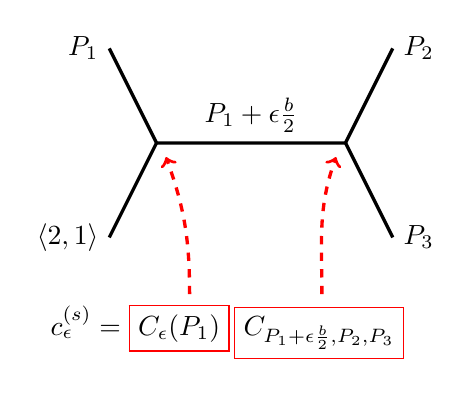
\begin{tikzpicture}[baseline=(current  bounding  box.center), very thick, scale = .6]
\draw (-1,2) node [left] {$P_1$} -- (0,0) -- node [above] {$P_1+\epsilon\frac{b}{2}$} (4,0) -- (5,2) node [right] {$P_2$};
\draw (-1,-2) node [left] {$\langle 2,1\rangle$} -- (0,0);
\draw (4,0) -- (5,-2) node [right] {$P_3$};
\node at (1.5, -4) {$c_{\epsilon}^{(s)} = \colorboxed{red}{C_\epsilon(P_1)}\, \colorboxed{red}{C_{P_1+\epsilon\frac{b}{2},P_2,P_3}}  $};
\draw[dashed, ->, red] (.7,-3.2) to [out=90, in=-70] (.2, -.3);
\draw[dashed, ->, red] (3.5,-3.2) to [out=90, in=-110] (3.8, -.3);
\end{tikzpicture} 
\label{cs}
\end{align}
Crossing symmetry and single-valuedness of the four-point function imply that the two structure constants $c_\pm^{(s)}$ obey eq. \eqref{eq:coc},
\begin{align}
 \frac{C_+(P_1) C_{P_1+\frac{b}{2},P_2,P_3}}{C_-(P_1) C_{P_1-\frac{b}{2},P_2,P_3} } 
 =\gamma(2bP_1) \gamma(1+2bP_1)\prod_{\pm,\pm} \gamma(\tfrac12 -bP_1 \pm bP_2 \pm bP_3)\ ,
 \label{eq:shift}
\end{align}
where we introduce the ratio of Euler Gamma functions
\begin{align}
 \gamma(x) = \frac{\Gamma(x)}{\Gamma(1-x)}\ .
\label{gx}
\end{align}
In order to find the three-point structure constant $C_{P_1,P_2,P_3}$, we need to constrain the degenerate OPE coefficients $C_\epsilon(P)$. To do this, we consider the special case where the last field is degenerate too, i.e. the four-point function $\Big\langle V_{\langle 2,1 \rangle}(z) V_P(0) V_{P}(\infty) V_{\langle 2,1 \rangle}(1)\Big\rangle$, and we find 
\begin{align}
 \frac{C_+(P)^2B(P+\tfrac{b}{2})}{C_-(P)^2 B(P-\tfrac{b}{2})}
 =  \frac{\gamma(2bP)}{\gamma(-2bP)}
 \frac{\gamma(-b^2-2bP)}{\gamma(-b^2+2bP)} \ .
 \label{eq:shiftd}
\end{align}
Moreover, if we had the degenerate field $V_{\langle 1,2\rangle}$ instead of $V_{\langle 2,1\rangle}$ in our four-point functions, we would obtain the equation \eqref{eq:shift} with $b\to \frac{1}{b}$.

In order to solve the shift equations for $C_{P_1,P_2,P_3}$, we need a function that produces Gamma functions when its argument is shifted by $b$ or $\frac{1}{b}$. More precisely, we need a function such that 
\begin{align}
  \frac{\Upsilon_b(x+b)}{\Upsilon_b(x)} = b^{1-2bx} \gamma(bx)\qquad \text{and} \qquad \frac{\Upsilon_b(x+\frac{1}{b})}{\Upsilon_b(x)} = b^{\frac{2x}{b}-1} \gamma(\tfrac{x}{b})\ ,
\label{upup}
\end{align}
where the prefactors ensure that the two shift equations are compatible with one another.  In the complex plane, the periods $b$ and $\frac{1}{b}$ indeed look as follows:
\begin{equation}
 \begin{tikzpicture}[baseline=(current  bounding  box.center), scale = .6]
\draw (0, 2) node[left]{$i$} -- (0, 1) node[below left] {$0$} -- (1, 1) node[below] {$1$};
\draw [red, thick, latex-latex] (11,3) -- (11,1) node[fill, circle, minimum size = 1mm, inner sep = 0]{} -- (11,-.3);
\draw [red, thick, latex-latex] (8,3) -- (7,1) node[fill, circle, minimum size = 1mm, inner sep = 0]{}-- (7.6,-.2);
\draw [red, thick, latex-latex] (5,1) -- (3,1) node[fill, circle, minimum size = 1mm, inner sep = 0]{} -- (4.3,1) ;
\node at (4, -1.5){$\begin{array}{c} b^2>0 \\ c\geq 25 \end{array}$};
\node at (7.5, -1.5){$\begin{array}{c} b\in \mathbb{C} \\ c\in\mathbb{C} \end{array}$};
\node at (11, -1.5){$\begin{array}{c} b^2<0 \\ c\leq 1 \end{array}$};
 \end{tikzpicture}
\end{equation}
The periods are aligned if $b^2\in \mathbb{R}-\mathbb{Q}$, so the solution is unique for these values of $b^2$. By analyticity in $b$, the unique solution for $b^2\in \mathbb{R}_{>0}-\mathbb{Q}$ can be extended to all $b^2\notin \mathbb{R}_{\leq 0}$,
\begin{align}
 \Upsilon_b(x) = \lambda_b^{(\frac{Q}{2}-x)^2}\prod_{m,n=0}^\infty f\left(\frac{\frac{Q}{2}-x}{\frac{Q}{2}+mb+nb^{-1}}\right) \quad \text{with} \quad f(x)=(1-x^2)e^{x^2}\ .
 \label{eq:up}
\end{align}
The unique solution for $b^2\in \mathbb{R}_{<0}-\mathbb{Q}$, which can be analytically extended to $b^2\notin \mathbb{R}_{\geq 0}$, is 
\begin{align}
 \hat{\Upsilon}_b(x) = \frac{1}{\Upsilon_{ib}(-ix+ib)}\ .
\end{align}

Let us now solve the shift equations \eqref{eq:shift} and \eqref{eq:shiftd} using the function $\Upsilon_b$:
\begin{align}
 C_{P_1,P_2,P_3} =  \frac{1}{\prod_{\pm,\pm} \Upsilon_b\left(\tfrac{Q}{2}+P_1\pm P_2 \pm P_3\right)} \ ,
 \label{cppp}
\end{align}
\begin{align}
 B(P) = \frac{1}{\prod_\pm \Upsilon_b(\pm 2P)}\ .
 \label{eq:ntbm}
\end{align}
This holds if $b^2\notin \mathbb{R}_{\leq 0}$ i.e. 
$c\notin ]-\infty, 1]$. 
On the other hand, doing the replacement $\Upsilon_b\to \hat\Upsilon_b$, we obtain a solution $\hat C$ that holds if $b^2\notin \mathbb{R}_{\leq 0}$ i.e. $c\notin [25,\infty[$.

\subsection{Existence and uniqueness}

For generic values of the central charge, both $C$ and $\hat C$ are solutions, and there are actually infinitely many other solutions. In order to prove the existence and uniqueness of Liouville theory, we have to determine which solutions lead to crossing-symmetric four-point functions. The $s$-channel 
decomposition of a Liouville four-point function is,
\begin{align}
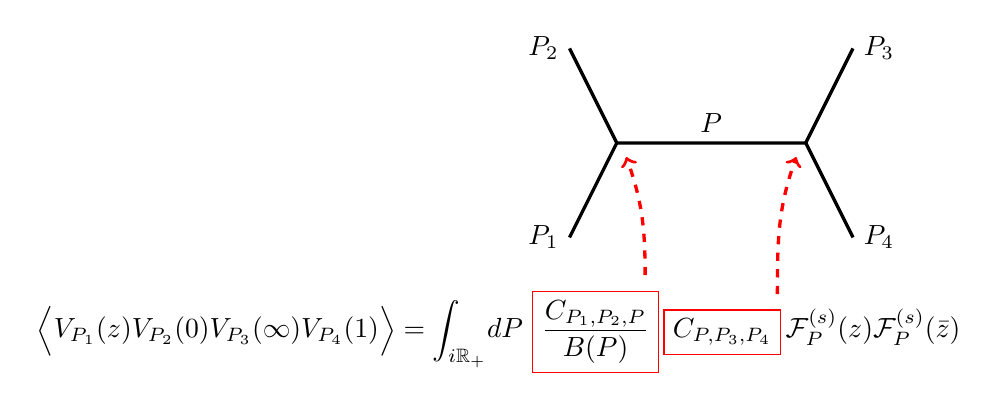
\begin{tikzpicture}[baseline=(current  bounding  box.center), very thick, scale = .6]
\draw (-1,2) node [left] {$P_2$} -- (0,0) -- node [above] {$P$} (4,0) -- (5,2) node [right] {$P_3$};
\draw (-1,-2) node [left] {$P_1$} -- (0,0);
\draw (4,0) -- (5,-2) node [right] {$P_4$};
\node at (-2.5, -4) {$\Big< V_{P_1}(z) V_{P_2}(0) V_{P_3}(\infty) V_{P_4}(1)\Big> = {\displaystyle\int_{i\mathbb{R}_+}} dP\ \colorboxed{red}{\frac{C_{P_1,P_2,P}}{B(P)}}\, \colorboxed{red}{ C_{P,P_3, P_4}}\, \mathcal{F}_{P}^{(s)}(z) \mathcal{F}_{P}^{(s)}(\bar z)$};
\draw[dashed, ->, red] (.6,-2.8) to [out=90, in=-70] (.2, -.3);
\draw[dashed, ->, red] (3.4,-3.2) to [out=90, in=-110] (3.8, -.3);
\end{tikzpicture} 
\end{align}
(We have a similar expression with $B,C \to \hat B,\hat C$ whenever the solutions $\hat B, \hat C$ exist.) 
It can be numerically checked that crossing symmetry is obeyed whenever Liouville theory is unique, i.e. for $b^2\in \mathbb{R}^*$. 
We may be tempted to deduce that it is also obeyed whenever $C$ and $\hat{C}$ are defined, by analyticity in $b$. However, while $C$ and $\hat{C}$ are analytic, the four-point function may not be analytic, as poles of the integrand may cross the integration line. 
It turns out that this does not prevent $C$ from being crossing-symmetric whenever it is defined. 
However, $\hat{C}$ is crossing symmetric only for $b^2<0$. 
This saves us from the embarrassment of having two different Liouville theories for some values of the central charge, and Liouville theory is uniquely defined for any $c\in\mathbb{C}$. 


\end{document}

